%!TEX root = ../report.tex

This chapter delves into the testing used for this project, including design and implementation specific details.

First, the purpose and method of testing are explored, followed by an overview of this method. The types of tests that have been undertaken in this project, and their design, are then illustrated. Finally, the testing environment is outlined, including details on the testing framework and how testing was performed.

\section{Purpose} {
\label{sec:testing_purpose}

	Software testing is performed to verify that a system successfully satisfies and implements the previously established user requirements. Another critical role of software testing is to locate and prevent defects created during the software development cycle. Ultimately, testing aims to provide information about the level of quality in a system, so developers can deliver a high quality product~\footnote{\bibentry{istqb2015testing}}.

}

\section{Method} {
\label{sec:testing_method}

	This project has utilised the behavioural specifications, detailed in Section~\ref{sec:behavioural_specifications}, from behaviour-driven development (BDD), while maintaining a Rapid Application Development approach throughout development. This method of testing couples the advantages of RAD development, discussed in Section~\ref{sec:methodology} with the BDD approach outlined in Section~\ref{sec:behaviour_driven_development} below.

	\subsection{Behaviour-driven development} {
	\label{sec:behaviour_driven_development}

		Behaviour-driven development is an agile software development technique that focuses on obtaining a clear understanding of the desired software behaviour~\footnote{\bibentry{rice2014bdd}}. It utilises an ubiquitous language, which is shared by software developers and management teams to extract and gather requirements, specifications and documentation~\footnote{\bibentry{bellware2015bdd}}\footnote{\bibentry{evans2004domain}}. An important aspect of BDD is that the tests are highly granular, which enables programmers to determine points of failure more easily. Furthermore, BDD tests the system requirements, outputs the results in a natural human-readable format and provides living, up-to-date documentation of each system component.

	}

	\subsection{Behavioural specifications} {
	\label{sec:behavioural_specifications}

		BDD specifies behaviour through \emph{user stories}, which define the scope and acceptance criteria of the feature being tested~\footnote{\bibentry{north2007story}}. A story template should contain all of the elements contained in the following template:

		\begin{verbatim}
			Title: a clear, explicit title describing the story
 
			Narrative:
			As a [role]
			I want [feature]
			So that [benefit]
			 
			Acceptance criteria: presented as scenarios
			 
			Scenario 1: Title

			Given [context]
			  And [some more context]
			When  [event]
			Then  [outcome]
			  And [another outcome]

	  		Scenario 2: ...
		\end{verbatim}

	}

}

\section{Testing types} {
\label{sec:testing_types}

	This project has undertaken the following types of testing:

	\begin{description}
		\item[Unit testing:] Validates the smallest components of a system, ensuring it handles known inputs and outputs correctly~\footnote{\bibentry{atlassian2015testing}}.
			\begin{itemize}
				\item Unit tests should verify that the application works under expected, boundary, and negative cases.
			\end{itemize}
		% \item[System testing:] Verifies that a completely integrated system meets its requirements~\parencite{geraci1991ieee}.
		\item[Performance testing:] Determines the reliability, responsiveness, scalability, stability and throughput of a system under a particular workload~\footnote{\bibentry{microsoft2015performance}}.
	\end{description}

	\todo{evaluate why I'm using these types}

	These tests have been performed 

}

\section{Test design} {
\label{sec:test_design}

	\todo{solid principle}

	% http://blog.stevensanderson.com/2009/08/24/writing-great-unit-tests-best-and-worst-practises/

	% http://www.codeproject.com/Articles/5772/Advanced-Unit-Test-Part-V-Unit-Test-Patterns#Pass/Fail Patterns2

	% http://stackoverflow.com/questions/3840125/useful-design-patterns-for-unit-testing-tdd

	% http://programmers.stackexchange.com/questions/153410/what-are-the-design-principles-that-promote-testable-code-designing-testable-c
	
}

\section{Environment} {
\label{sec:testing_environment}

	The libraries used for the testing environment of this project have been outlined in Table~\ref{tab:testing_environment}.

	%!TEX root = ../report.tex

\begin{table}[H]
\caption[Testing environment]{The list of testing libraries used in the testing environment.}
\label{tab:testing_environment}
\begin{tabularx}{\textwidth}{@{}XX@{}}
	\toprule
	\textbf{Library} & \textbf{Description} \\
	\midrule
	Mocha & Testing framework \\
	Chai & Behaviour-driven development assertions \\
	Chai as promised & Promise assertions \\
	Sinon-chai & Spies, stubs and mocks \\
	Blanket & Code coverage \\
	Selenium & Automated browser testing \\
	\bottomrule
\end{tabularx}
\end{table}

}

\section{Testing framework} {
\label{sec:testing_framework}

	A testing framework is an execution environment for automated tests. They are responsible for defining a format to express expectations, test execution and reporting the results. Testing frameworks are application independent, easy to expand, maintain and are designed to help organise test suites to improve the efficiency of testing~\footnote{\bibentry{ghanakota2012testing}}.

	\subsection{Choosing a testing framework} {
	\label{sec:choosing_a_testing_framework}

		There are many popular JavaScript testing frameworks available such as Intern, Jasmine, Mocha and QUnit which have been assessed below.

		\emph{Intern} supports functional testing, has a very simple setup and great user interface which has been highlighted in Figure~\ref{fig:intern}. It became challenging to locate a code coverage library that could be integrated with Intern, since it was released in \href{https://github.com/theintern}{2013} and has less overall support. When testing out this framework, it was extremely difficult to run custom configurations before test execution, since configurations were not particularly flexible. This also meant that it was challenging to run tests with the correct RequireJS dependencies, since Intern uses the Dojo AMD loader by default.

		%!TEX root = ../../report.tex

\begin{figure}[H]
	\centering
    \figureborder{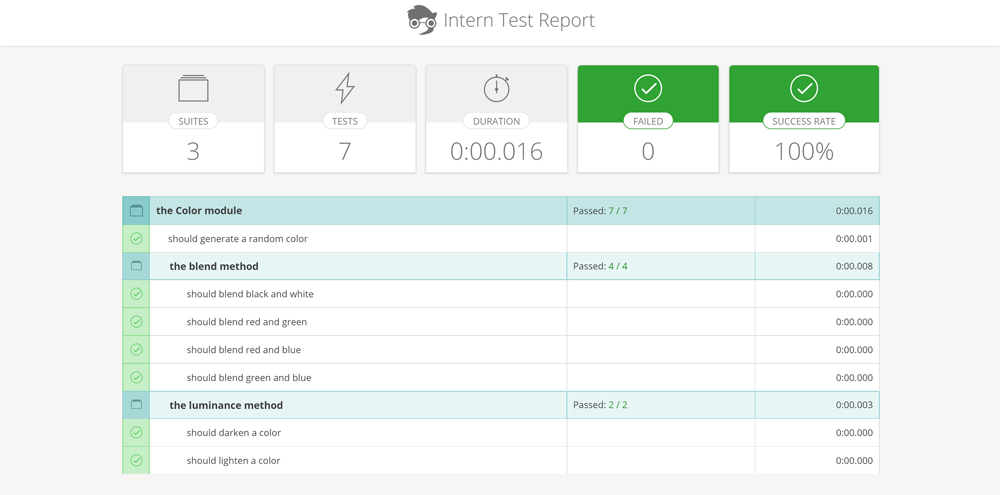
\includegraphics[width=\textwidth]{images/testing/intern}}
    \caption[Intern]{Intern user interface.}
    \label{fig:intern}
\end{figure}


		\emph{Jasmine} is often recommended and regarded as the most popular JS unit testing framework~\footnote{\bibentry{feldman2014testing}}. It has a simple setup, built-in assertions, is well supported, can adapt to other assertion libraries and performs code coverage when used with Istanbul. Jasmine also has an elegant, descriptive syntax that adheres to the BDD paradigm. However, its asynchronous testing support could be improved greatly, which is problematic for this particular project because asynchronous loading is used extensively.

		\emph{Mocha} proved to have a very simple setup, is highly extensible, very flexible, has good reporting and a BDD syntax that resembles Jasmine. It allows the use of any assertion library, enabling users to choose their preferred BDD style and offers great asynchronous testing and promise support. Mocha can also be integrated easily with Blanket, a code coverage tool. One issue with Mocha is that it has an overly simple and plain user interface, sometimes making it difficult to determine which tests have passed or failed.

		\emph{QUnit} was immediately discarded since it does not support the BDD paradigm, and instead utilises TDD.

		From these testing frameworks, \emph{Mocha} was chosen simply because of its fantastic asynchronous testing support and flexibility in choosing an assertion library and BDD style. Its user interface was transformed using customised CSS, which has been demonstrated in Figure~\ref{fig:mocha_styling}, so the tests become more readable.

		%!TEX root = ../../../report.tex

\newcommand{\mochawidth}{0.496\textwidth}
\newcommand{\mochaheight}{4cm}
\begin{figure}[H]
	\centering
	\begin{subfigure}[b]{\mochawidth}
        \figureborder{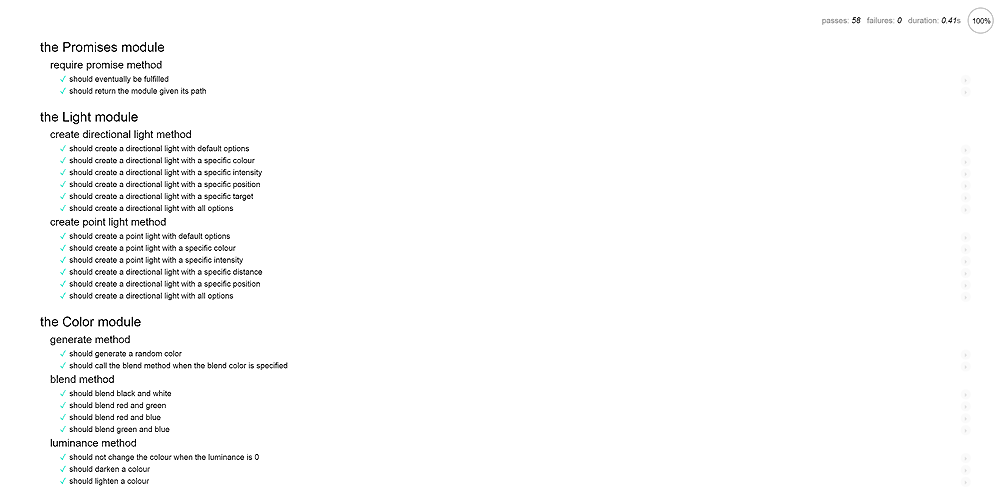
\includegraphics[width=\textwidth,height=\mochaheight]{images/testing/mocha_before}}
        \caption{Default Mocha interface.}
        \label{fig:mocha_before}
    \end{subfigure}
    \begin{subfigure}[b]{\mochawidth}
        \figureborder{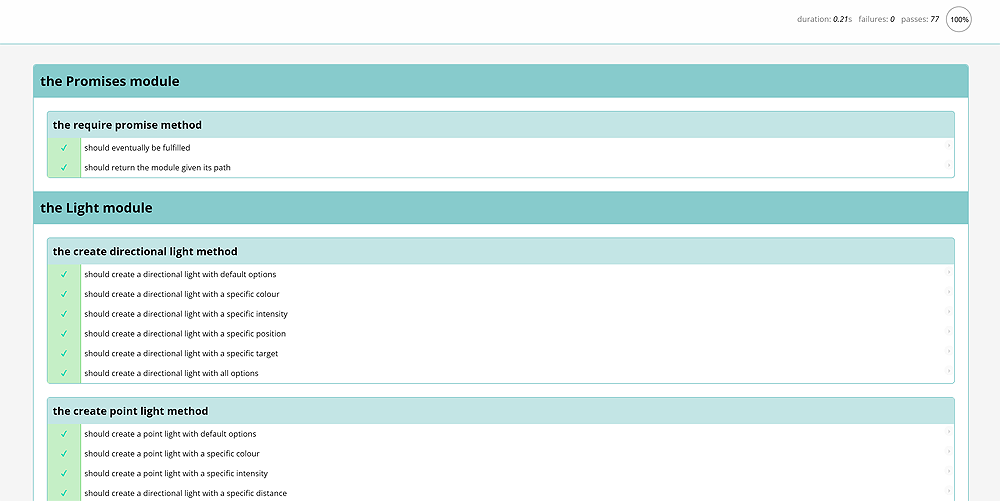
\includegraphics[width=\textwidth,height=\mochaheight]{images/testing/mocha_after}}
        \caption{Mocha interface after custom styling}
        \label{fig:mocha_after}
    \end{subfigure}
	\caption[Mocha]{Mocha styling}
	\label{fig:mocha_styling}
\end{figure}


	}

}

\section{Assertions} {
\label{sec:assertions}

	\emph{Chai} assertions were used with the Mocha testing framework, as they offer great flexibility. Users are able to choose their preferred BDD style, which has been illustrated in Figure~\ref{fig:chai_assertions}.

	%!TEX root = ../../../report.tex

\begin{figure}[H]
	\newcommand{\figurewidth}{0.325\textwidth}
	\newcommand{\basicstyle}{\tiny}
    \captionsetup[subfigure]{aboveskip=0em,belowskip=-0.2em}
	\begin{subfigure}[b]{\figurewidth}
        \centering
        %!TEX root = ../../../report.tex

\begin{lstlisting}[basicstyle=\basicstyle]
	chai.should();

	foo.should.be.a('string');
	foo.should.equal('bar');
	foo.should.have.length(3);
\end{lstlisting}

        \caption{Should style}
        \label{fig:should_style}
    \end{subfigure}
    \begin{subfigure}[b]{\figurewidth}
        \centering
    	%!TEX root = ../../../report.tex

\begin{lstlisting}[basicstyle=\basicstyle]
	var expect = chai.expect;
		
	expect(foo).to.be.a('string');
	expect(foo).to.equal('bar');
	expect(foo).to.have.length(3);
\end{lstlisting}

        \caption{Expect style}
        \label{fig:expect_style}
    \end{subfigure}
    \begin{subfigure}[b]{\figurewidth}
        \centering
		%!TEX root = ../../../report.tex

\begin{lstlisting}[basicstyle=\basicstyle]
    var assert = chai.assert;

	assert.typeOf(foo, 'string');
	assert.equal(foo, 'bar');
	assert.lengthOf(foo, 3)
\end{lstlisting}

        \caption{Assert style}
        \label{fig:assert_style}
    \end{subfigure}
	\caption[Chai assertions]{Chai assertion styles.}
	\label{fig:chai_assertions}
\end{figure}


	The \emph{should} style adheres to BDD and its behavioural specifications. However, this style extends \texttt{Object.prototype} which is generally considered bad practice. This style is not compatible in all browsers and results in scenarios where a test can fail~\footnote{\bibentry{luer2015assertion}}. Instead, the \emph{expect} style was used because it is compatible across all browsers and utilises chainable, natural language assertions. This style closely resembles BDD specifications, unlike the \emph{assert} style.

	\subsection{Asynchronous support} {
	\label{sec:testing_asynchronous_support}

		Mocha provides a way to test asynchronous code through the \texttt{done} callback or by returning a \texttt{Promise}~\footnote{\bibentry{holowaychuk2011mocha}}, which has been presented in Figure~\ref{fig:mocha_asynchronous_code}. Promises are used extensively when loading shaders, so it was important to have a clean way of testing asynchronous code. 

		%!TEX root = ../../../report.tex

\begin{figure}[H]
	\newcommand{\basicstyle}{\scriptsize}
	\begin{subfigure}[b]{0.45\textwidth}
        %!TEX root = ../../../report.tex

\begin{lstlisting}[basicstyle=\basicstyle]
	doSomethingAsync()
		.then(function (result) {
			result.should.equal('foo');
			done();
		}
	);
\end{lstlisting}

        \caption{Callback}
        \label{fig:mocha_callback}
    \end{subfigure}
    \begin{subfigure}[b]{0.5\textwidth}
		%!TEX root = ../../../report.tex

\begin{lstlisting}[basicstyle=\basicstyle]
	return doSomethingAsync()
		.then(function (result) {
			// Return the result from the promise.
			return result.should.equal('foo');
		}
	);
\end{lstlisting}

        \caption{Promise}
        \label{fig:mocha_promise}
    \end{subfigure}
	\caption[Mocha asynchronous code]{Mocha asynchronous code.}
	\label{fig:mocha_asynchronous_code}
\end{figure}


		However, this method of testing asynchronous code could be improved by using the \emph{Chai as Promised} plugin for Chai. This plugin extends Chai with a fluent language for asserting facts about promises~\footnote{\bibentry{denicola2012chaiaspromised}}. An example of this improvement has been illustrated in Figure~\ref{fig:chai_as_promised}, which transforms the assertion seen in Figure~\ref{fig:mocha_asynchronous_code} down to one line.

		%!TEX root = ../../../report.tex

\begin{figure}[H]
	\centering
	\begin{lstlisting}
		return doSomethingAsync().should.eventually.equal('foo');
	\end{lstlisting}
	\caption[Chai as Promised]{Chai as Promised.}
    \label{fig:chai_as_promised}
\end{figure}


	}

	\subsection{Spies, stubs and mocks} {
	\label{sec:testing_spy_stub_mock_support}

		Mocha is not equipped with spies, stubs or mocks~\footnote{\bibentry{holowaychuk2011mocha}} and instead recommend using \emph{Sinon.JS}, a popular library designed for this purpose. Similarly to Section~\ref{sec:testing_asynchronous_support}, a plugin called \emph{Sinon-Chai} provides a set of custom assertions for using the Sinon.JS spy, stub, and mocking framework with the Chai assertion library~\footnote{\bibentry{denicola2012sinonchai}}.

	}

}

\section{General structure} {
\label{sec:testing_structure}

	In Mocha, the \texttt{describe} keyword is a way to group tests together, while each \texttt{it} clause represents a single test case. A simple example of a test suite has been shown in Figure~\ref{fig:mocha_example}.

	%!TEX root = ../../../report.tex

\begin{figure}[H]
	\centering
	%!TEX root = ../../../report.tex

\begin{figure}[H]
	\centering
	%!TEX root = ../../../report.tex

\begin{figure}[H]
	\centering
	\input{code/testing/mocha/example}
	\caption[Mocha example]{Mocha example.}
	\label{fig:mocha_example}
\end{figure}

	\caption[Mocha example]{Mocha example.}
	\label{fig:mocha_example}
\end{figure}

	\caption[Mocha example]{Mocha example.}
	\label{fig:mocha_example}
\end{figure}


}

\section{Hooks} {
\label{sec:testing_hooks}

	Mocha provides \texttt{before}, \texttt{after}, \texttt{beforeEach} and \texttt{afterEach} hooks, which are described in Figure~\ref{fig:mocha_hooks}. These hooks can be used to set up preconditions or to perform test clean up~\footnote{\bibentry{holowaychuk2011mocha}}.

	\begin{figure}[H]
	\centering
	\begin{lstlisting}
		describe('hooks', function () {

			before(function () {
				// runs before all tests in this block
			});

			after(function () {
				// runs after all tests in this block
			});

			beforeEach(function () {
				// runs before each test in this block
			});

			afterEach(function () {
				// runs after each test in this block
			});

			// test cases

		});
	\end{lstlisting}
	\caption[Mocha hooks]{Mocha hooks.}
	\label{fig:mocha_hooks}
\end{figure}


	Typically, \texttt{beforeEach} and \texttt{afterEach} hooks were used when running tests to:

	\begin{itemize}
		\item Initialize shared variables.
		\item Create spies or stubs for methods that were called in each test suite.
		\item Perform common assertions after initialising a test case.
		\item Reset stubs or other data.
	\end{itemize}

}

\section{Style} {
\label{sec:testing_style}

	The style used throughout the Mocha documentation resembles Figure~\ref{fig:mocha_example} where the following is true:

	\begin{itemize}
		\item The top level \texttt{describe} represents the class name.
		\item Any proceeding \texttt{describe} clauses represent the method name in the form of \texttt{\#methodName()}.
		\item Each sentence in a test case may or may not be preceeded by \texttt{should}.
	\end{itemize}

	This style was therefore found to be quite inconsistent and does not output the results in a human-readable format. Instead, the following style was developed and used when developing tests:

	\begin{itemize}
		\item The top level \texttt{describe} represents the name of the AMD module and reads as \texttt{the ModuleName module}.
			\begin{itemize}
				\item Preceeding the module name with the word \texttt{the} adheres to the behavioural specifications, by following a fluid sentence structure.
			\end{itemize}
		\item Any proceeding \texttt{describe} clauses represent the method name in the form of \texttt{methodName method}.
			\begin{itemize}
				\item Adding \texttt{method} to the end of each title makes the test case more human-readable.
			\end{itemize}
		\item Each sentence in a test case is preceeded by \texttt{should}.
	\end{itemize}

	An example of this style has been demonstrated in Figure~\ref{fig:testing_style}.

	%!TEX root = ../../report.tex

\begin{figure}[H]
	\centering
	%!TEX root = ../../report.tex

\begin{figure}[H]
	\centering
	%!TEX root = ../../report.tex

\begin{figure}[H]
	\centering
	\input{code/testing/style}
	\caption[Testing style]{Testing style.}
	\label{fig:testing_style}
\end{figure}

	\caption[Testing style]{Testing style.}
	\label{fig:testing_style}
\end{figure}

	\caption[Testing style]{Testing style.}
	\label{fig:testing_style}
\end{figure}


}

% \section{Example} {
% \label{sec:testing_examples}

% 	%!TEX root = ../../../report.tex

\begin{figure}[H]
	\centering
	%!TEX root = ../../../report.tex

\begin{figure}[H]
	\centering
	%!TEX root = ../../../report.tex

\begin{figure}[H]
	\centering
	\input{code/testing/mocha/example}
	\caption[Mocha example]{Mocha example.}
	\label{fig:mocha_example}
\end{figure}

	\caption[Mocha example]{Mocha example.}
	\label{fig:mocha_example}
\end{figure}

	\caption[Mocha example]{Mocha example.}
	\label{fig:mocha_example}
\end{figure}


% }

\section{Code coverage} {
\label{sec:code_coverage}

	Code coverage is the measurement of how many lines of code are executed while automated tests are running, making it a useful tool for finding untested code. Take the following snippet of code as an example:

	%!TEX root = ../../report.tex

\begin{lstlisting}
	if (condition) {
		// True condition - first branch
	} else {
		// False condition - second branch
	}
\end{lstlisting}


	If the \texttt{condition} is always \texttt{true}, then the second branch will never execute. Therefore, the unit test does not cover the false branch and this will be displayed in the results of a code coverage. Tests would ideally cover \textgreater80\% for a single test suite.

	\href{http://blanketjs.org/}{Blanket.js} was used in this project as a code coverage tool because it seamlessly integrates with Jasmine, Mocha and QUnit. Blanket injects the code coverage results at the bottom of the HTML page, which has been demonstrated in Figure~\ref{fig:blanket}.

	\begin{figure}[H]
	\centering
    \figureborder{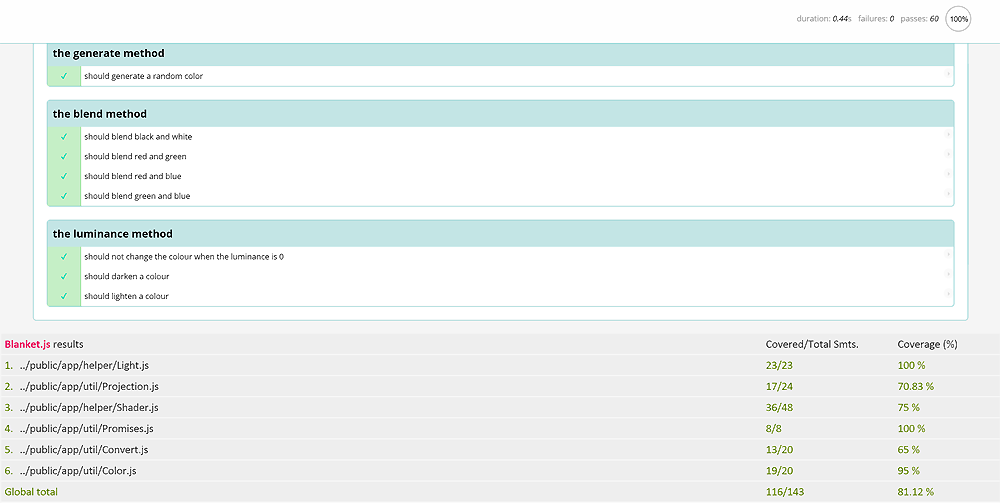
\includegraphics[width=\textwidth]{images/testing/blanket}}
    \caption[Blanket]{Blanket code coverage.}
    \label{fig:blanket}
\end{figure}


	A result from the code coverage can be expanded to reveal more information. It displays the entire file, including line numbers, and highlights the lines of code that were not covered under the tests that were executed. This behaviour can be identified in Figure~\ref{fig:code_coverage_results}, which demonstrates a method that was not tested.

	\begin{figure}[H]
	\centering
    \figureborder{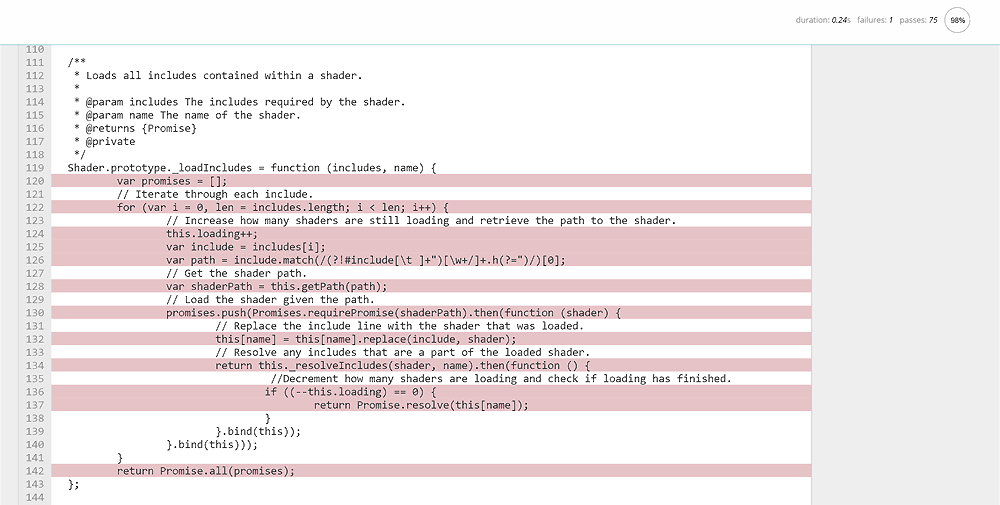
\includegraphics[width=\textwidth]{images/testing/coverage_results}}
    \caption[Code coverage results]{Code coverage results.}
    \label{fig:code_coverage_results}
\end{figure}


	Code coverage was evaluated after the creation of each test suite. When a test suite was analysed, more tests would be written in an attempt to improve the overall code coverage. This process was repeated until an acceptable amount of code coverage was reached.

}

\section{Performance testing} {
\label{sec:performance_testing}

	\todo{Introduce setup - selenium}

}
